\documentclass{article}
\usepackage{tikz}

\begin{document}

\begin{figure}[h]
    \centering
    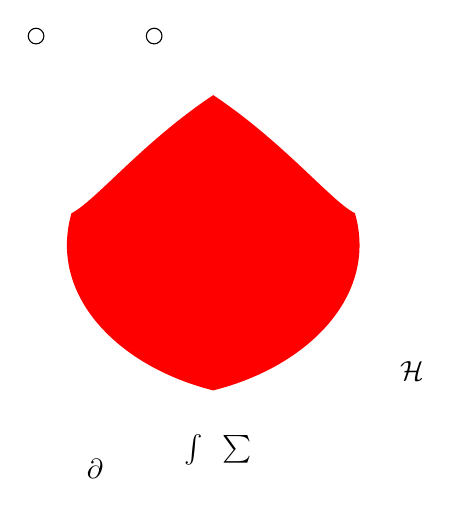
\begin{tikzpicture}[scale=1.5]

        % Draw the heart
        \fill[red] (0,0) .. controls (-0.6,-0.4) and (-1,-0.9) .. (-1.2,-1)
                    .. controls (-1.4,-1.7) and (-0.8,-2.3) .. (0,-2.5)
                    .. controls (0.8,-2.3) and (1.4,-1.7) .. (1.2,-1)
                    .. controls (1,-0.9) and (0.6,-0.4) .. cycle;

        % Place the birds
        \node[circle, fill=white, draw=black, inner sep=2pt] at (-1.5, 0.5) {};
        \node[circle, fill=white, draw=black, inner sep=2pt] at (-0.5, 0.5) {};

        % Placeholder mathematical symbols
        \node[above right] at (1.5, -2.5) {$\mathcal{H}$};
        \node[left] at (0, -3) {$\int$};
        \node[right] at (0, -3) {$\sum$};
        \node[below] at (-1, -3) {$\partial$};

    \end{tikzpicture}
    \caption{Heart with two birds and surrounding mathematical symbols}
    \label{fig:heart_birds_symbols}
\end{figure}

\end{document}